% !TEX root = mythesis.tex



%==============================================================================
\chapter{Uncertainties}
\label{sec:uncertainty_result}
%==============================================================================
The purpose of this chapter is to discuss all the uncertainties taken into account for the multijet estimation. It includes both the statistical and systematic uncertainties. A detailed procedure for the calculation of different systematic uncertainties and their individual contribution to the estimated multijet is also described in detail. 
%==============================================================================
\section{Statistical uncertainties}
\label{sec:uncertainties:statistical}
%==============================================================================
Statistical uncertainties can reliably be estimated by repeating measurements. If the sample follows the Poisson distribution, then the statistical uncertainty reduces to $1/\sqrt{N}$ where $N$ is the sample size. When a histogram is filled with events, the statistical uncertainty associated with each bin of a histogram is given by $\sqrt{\text{bin content}}$. When the arithmetic operations are performed between the histograms, the statistical uncertainties propagate and follow the Gaussian error propagation. 

In this thesis, the statistical uncertainties are arising from two different sources: first from the ABCD method where the arithmetic operations (like subtraction, multiplication and division) are performed between the histograms according to the ABCD equation shown in \ref{eqn:abcd:correctionfactor}. In this, the statistical uncertainty in each bin of the distributions propagates by Gaussian error propagation and contributes to the estimated multijet distribution.

The other statistical uncertainty arises from the calculation of \R. In this, the likelihood fit is performed to fit the multijet MC to the data, and the output of the fit, which is the scaled multijet MC is used to calculate \R. The statistical uncertainty in the distribution of the scaled multijet MC contributes less because the fit constrains the uncertainty associated with each bin. However, when the arithmetic operations are performed on the scaled multijet MC for the calculation of \R, the uncertainties in each bin of the distribution follow the Gaussian error propagation and contribute further to the statistical uncertainty. A detailed contribution of the total statistical uncertainty to the multijet estimate in all the distributions is given in Table \ref{table:uncertainties:systematics:detail}.
%==============================================================================
\section{Systematic uncertainties}
\label{sec:uncertainties:systematics}
%==============================================================================
Systematic uncertainties are the ones which are not directly due to the statistics of the sample. They can arise from any source, for example, limited knowledge of backgrounds or the badly modelled backgrounds. Sometimes, they can also come from the imperfect detector resolutions or some other external factors affecting the detector acceptance. In general, they are difficult to determine because they cannot be calculated solely from the sampling fluctuations. So, different approaches have to be performed in order to estimate various systematic uncertainties. They are broadly divided into three categories:

First is theoretical uncertainties which arise from the theoretical prediction of different observables. The choice of the MC generator and their parameters are empirical for modelling the signal and background samples. So, different choices lead to different results which can affect the measurement. It includes uncertainties on the calculation of the matrix element, uncertainty on the parton shower and the hadronisation process, correction of different radiation levels (like initial- and final-state radiation), uncertainty due to the choice of the parton distribution function etc. A general procedure to estimate the uncertainties which depend on the choice of a generator is to replace a generator by another one or vary the values of the parameters, and simulate full samples again and then evaluate their contribution to the uncertainty.

Second is detector and algorithm performances uncertainties which arise from the imperfect detector and reconstruction algorithms, which are usually studied by the various performance groups in ATLAS. These include uncertainties associated with different efficiencies, trigger and scale factors. It also consists of inaccuracy in energy calibration and the measurement of jet energy scale and jet energy resolution. Uncertainties in the reconstruction and tagging algorithms also contribute a lot, especially when $b$-tagging is used in the analysis. The procedure of estimating these uncertainties might differ depending on the analysis.

The third is luminosity and cross-section uncertainties. One should assume uncertainty on luminosity since the luminosity is also not always constant throughout the data taking period, and there might be some fluctuations which need to be taken into account. The various modelling groups in ATLAS usually give the uncertainty on the theoretical values of the cross-section of different processes which needs to be taken into account in the analysis.

The contribution from these uncertainties leads to one of the two possible types of effects on the distributions. The first one is normalisation and shape effect that means some uncertainties (when taken into account) leads to a difference in the event yields as well as fluctuations in the shape of the distribution. The second one is shape only effect where one can only see the difference in the shape of the distribution without any change in the total number of events. Although it does not affect the measurement (or the multijet estimate in this case), it is important to consider this type of uncertainty when comparing an estimate with the data at the distribution level.

Due to limited time and availability of the MC samples, the study of all the systematic uncertainties is not feasible, where some of them are even beyond the scope of this thesis.  So, the systematic uncertainties which are studied in this thesis are described in detail below:

%==============================================================================
\subsection{$b$-tagging uncertainty}
\label{sec:uncertainties:systematics:btagging}
%==============================================================================
In this thesis, the estimation of multijet relies on the choice of two uncorrelated variables where one of the variables is $b$-jet multiplicity. The tagging of jets which are actually originating from the decay of $b$-quark is purely objective because sometimes the $b$-tagging algorithm mistagged $c$-jets and other light flavoured jets as $b$-jets.  So, in that case, the uncertainty associated with the performance of the $b$-tagging algorithm has to be taken into account.

The $b$-tagging uncertainties are estimated by varying five parameters in the MC simulation, which contributes the most. These parameters affect the $b$-tagging scale factor, which changes the $b$-tagging weight $w_{\text{b-tagging}}$ in Eqn.\ \ref{eqn:analysisstrategy:mc:weights}. And these weights are then applied to the events of all MC simulated backgrounds to calculate the total event yield.

The $b$-tagging uncertainty has been implemented by changing all the five parameters one by one in the MC simulation of all the backgrounds. For each of the parameters, first the MC is simulated by taking up variation and then by taking the down variation into account. So that means, in total, ten different MC samples for all the backgrounds are produced (five for both up and down variations). Then, the ABCD method is performed by using each of these MC background samples one by one, and the multijet background is estimated in the validation region. The multijet estimate varies in all these ten cases because the MC backgrounds have different $b$-tagging weights in all these cases (because of the change in the parameter). The difference in the normalisation of each of these ten multijet estimates with the final multijet estimate is taken as the $b$-tagging uncertainty. Since both the up and down variations of five parameters are taken into account, so the absolute mean of them is taken into account. 

The five parameters which are varied to calculate the $b$-tagging uncertainty are described in detail below along with their individual contribution towards the $b$-tagging uncertainty:

\begin{itemize}
	\item \textit{eigenvars\_b:} the scale factors are applied in order to correct for mismodelling in the output of the $b$-tagging algorithm. These scale factors are derived separately for $b$-jets, $c$-jets and light-flavour jets. Using an eigenvector decomposition~\cite{btagging:uncertainties}, these uncertainties are decomposed into different eigenvectors of $b$-jets, $c$-jets and light-flavoured jets. \textit{eigenvars\_b} is defined as the eigenvectors for $b$-jet efficiency. Fig.\ \ref{fig:uncertainties:systematics:btagging:b} shows the contribution of uncertainty from the eigenvector of $b$-jet efficiency in \pt distribution of the leading $b$-jet and VLQ mass. It can be observed that this uncertainty does not contribute much to the normalisation difference but contributes towards the shape difference.
	\begin{figure}[hbt!]
		\centering
		\graphicspath{{figs/chapter6/Systematics/EigenvarsB/}}
		\begin{subfigure}{.35\textwidth}
			\centering
			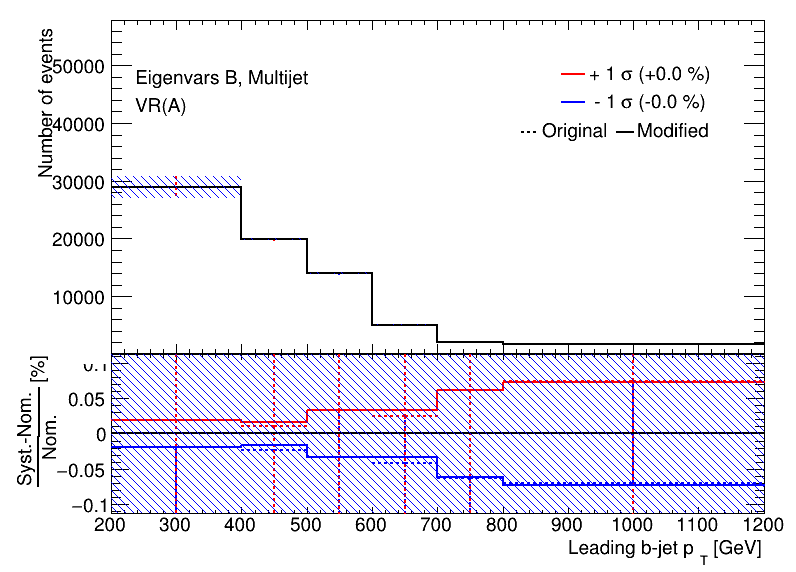
\includegraphics[width=\linewidth,height=\textheight,keepaspectratio]{VR_B_jet_pt_Multijets.png}
			\caption{}
			\label{fig:uncertainties:systematics:btagging:b:jetpt}
		\end{subfigure}\hspace{0.6cm}
		\begin{subfigure}{.35\textwidth}
			\centering
			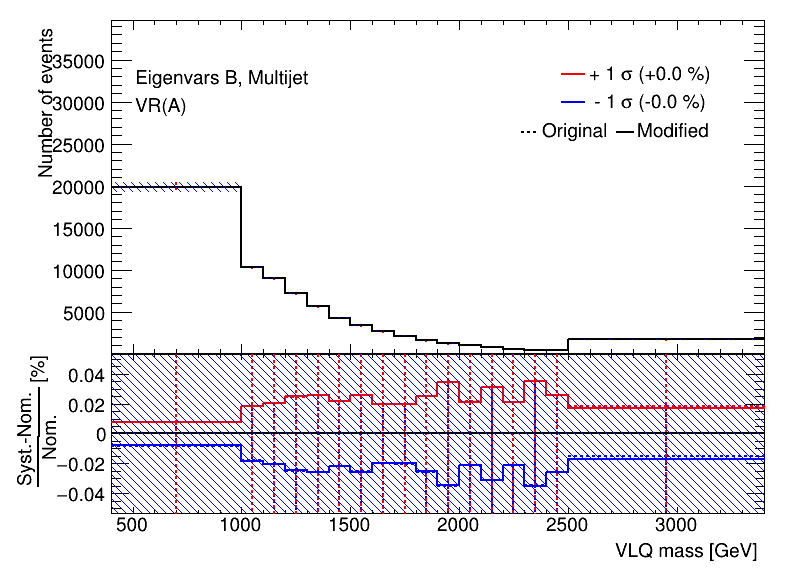
\includegraphics[width=\linewidth,height=\textheight,keepaspectratio]{VR_B_VLQM_Multijets.png}
			\caption{}
			\label{fig:uncertainties:systematics:btagging:b:vlqm}
		\end{subfigure}
		\caption{Comparison between the Systematics-Nominal and Nominal, where Systematics-Nominal denotes the estimated multijet when both up (in red) and down (in blue) variations in \textit{eigenvars\_b} are taken into account, and Nominal denotes the final estimated multijet (in black). The difference between the two is considered as the systematic uncertainty from the eigenvectors of the $b$-jet efficiency. It is shown for (a) leading $b$-tagged jet \pt and (b) VLQ mass distribution.}
		\label{fig:uncertainties:systematics:btagging:b}
	\end{figure}

	\item \textit{eigenvars\_c:} it is defined as the eigenvectors for $c$-jets which describes the scale factors of $c$-jets mistagged as $b$-jets. Fig.\ \ref{fig:uncertainties:systematics:btagging:c} shows the contribution of uncertainty from the eigenvector of $c$-jet efficiency in \pt distribution of the leading $b$-jet and VLQ mass. One can see that \pt distribution shows 0.1\% difference in the normalisation of the distribution, whereas VLQ mass distribution only contributes to the difference in the shape of the distribution.
	\begin{figure}[hbt!]
		\centering
		\graphicspath{{figs/chapter6/Systematics/EigenvarsC/}}
		\begin{subfigure}{.35\textwidth}
			\centering
			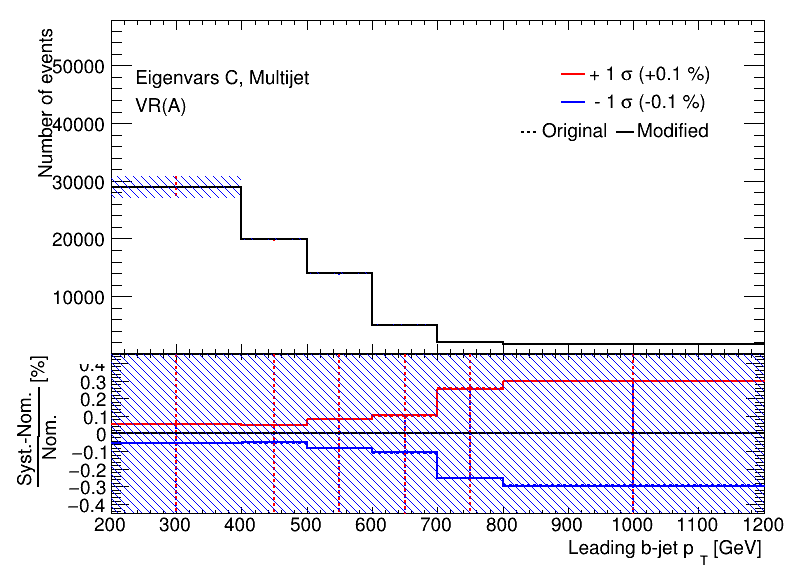
\includegraphics[width=\linewidth,height=\textheight,keepaspectratio]{VR_B_jet_pt_Multijets.png}
			\caption{}
			\label{fig:uncertainties:systematics:btagging:c:jetpt}
		\end{subfigure}\hspace{0.6cm}
		\begin{subfigure}{.35\textwidth}
			\centering
			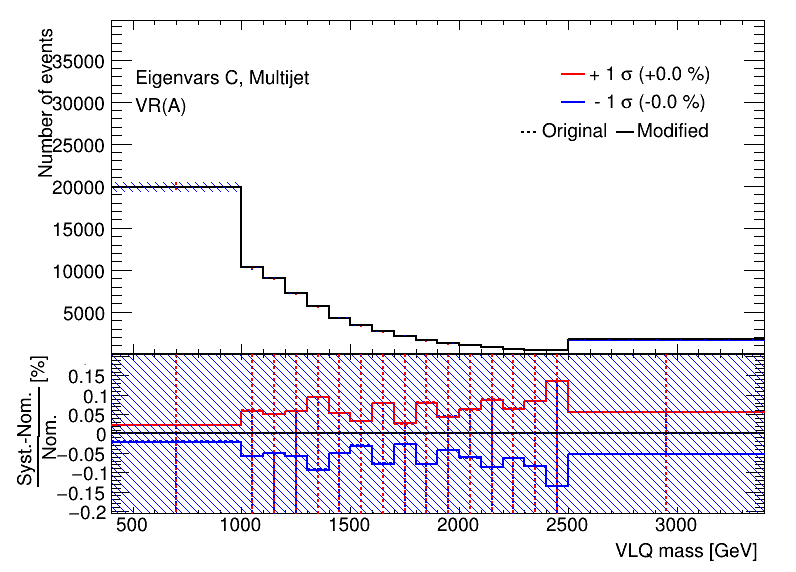
\includegraphics[width=\linewidth,height=\textheight,keepaspectratio]{VR_B_VLQM_Multijets.png}
			\caption{}
			\label{fig:uncertainties:systematics:btagging:c:vlqm}
		\end{subfigure}
		\caption{Comparison between the Systematics-Nominal and Nominal, where Systematics-Nominal denotes the estimated multijet when both up (in red) and down (in blue) variations in \textit{eigenvars\_c} are taken into account, and Nominal denotes the final estimated multijet (in black). The difference between the two is considered as the systematic uncertainty from the eigenvectors of $c$-jets. It is shown for (a) leading $b$-tagged jet \pt and (b) VLQ mass distribution.}
		\label{fig:uncertainties:systematics:btagging:c}
	\end{figure}

	\item \textit{eigenvars\_light:} it is defined as the eigenvectors for light-flavoured jets which describes the scale factors of light-flavoured jets mistagged as $b$-jets. Fig.\ \ref{fig:uncertainties:systematics:btagging:light} shows the contribution of uncertainty from the eigenvector of light-flavoured jet in \pt distribution of the leading $b$-jet and VLQ mass. It contributes to the difference in the normalisation of all the kinematic distributions except the $\eta$ distribution.
	\begin{figure}[hbt!]
		\centering
		\graphicspath{{figs/chapter6/Systematics/EigenvarsLight/}}
		\begin{subfigure}{.35\textwidth}
			\centering
			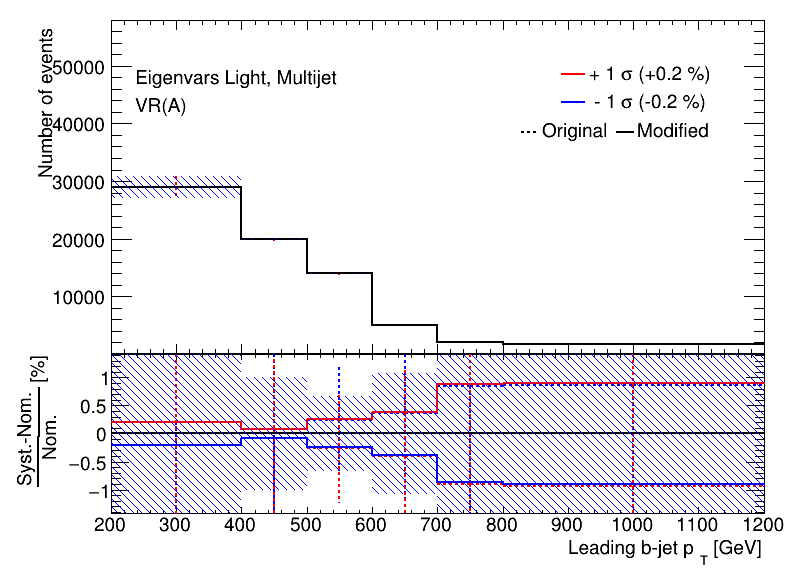
\includegraphics[width=\linewidth,height=\textheight,keepaspectratio]{VR_B_jet_pt_Multijets.png}
			\caption{}
			\label{fig:uncertainties:systematics:btagging:light:jetpt}
		\end{subfigure}\hspace{0.6cm}
		\begin{subfigure}{.35\textwidth}
			\centering
			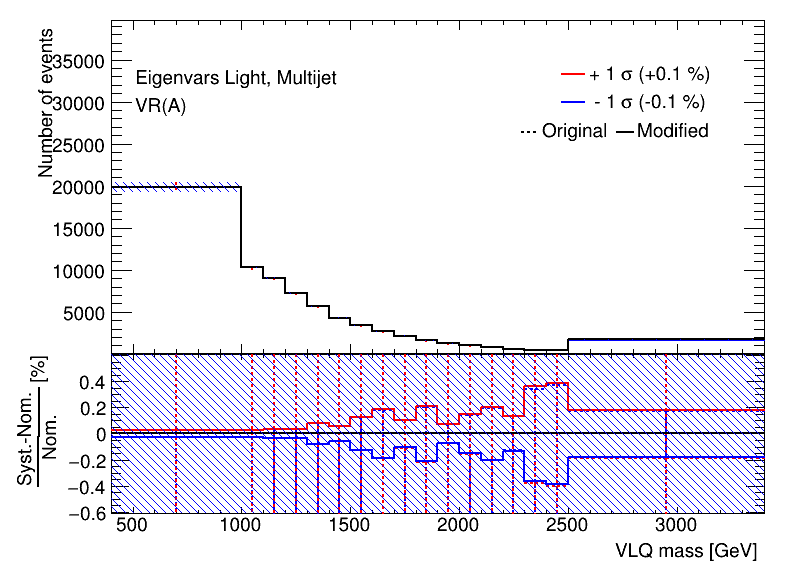
\includegraphics[width=\linewidth,height=\textheight,keepaspectratio]{VR_B_VLQM_Multijets.png}
			\caption{}
			\label{fig:uncertainties:systematics:btagging:light:vlqm}
		\end{subfigure}
		\caption{Comparison between the Systematics-Nominal and Nominal, where Systematics-Nominal denotes the estimated multijet when both up (in red) and down (in blue) variations in \textit{eigenvars\_light} are taken into account, and Nominal denotes the final estimated multijet (in black). The difference between the two is considered as the systematic uncertainty from the eigenvectors of light-flavoured jets. It is shown for (a) leading $b$-tagged jet \pt and (b) VLQ mass distribution.}
		\label{fig:uncertainties:systematics:btagging:light}
	\end{figure}

	\item \textit{extrapolation}: the precise measurement of $b$-tagging efficiency for jets is only implemented up to a certain jet \pt. The evaluation of the uncertainty in $b$-tagging efficiency beyond this \pt range can be calculated by \textit{extrapolation}, which describes the extrapolation uncertainties of \pt.~\cite{btagging:uncertainties} Fig.\ \ref{fig:uncertainties:systematics:btagging:extra} shows the contribution of the extrapolation uncertainty in \pt distribution of the leading $b$-jet and VLQ mass.
	\begin{figure}[hbt!]
		\centering
		\graphicspath{{figs/chapter6/Systematics/Extrapolation/}}
		\begin{subfigure}{.35\textwidth}
			\centering
			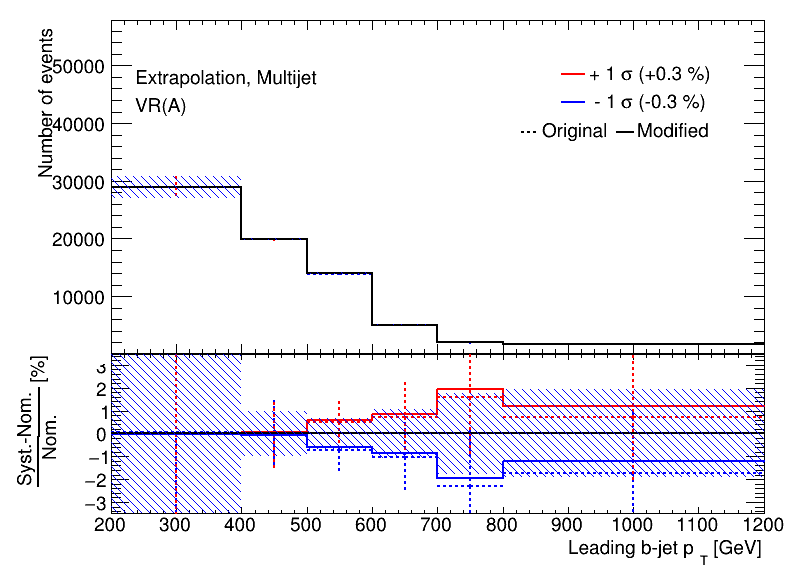
\includegraphics[width=\linewidth,height=\textheight,keepaspectratio]{VR_B_jet_pt_Multijets.png}
			\caption{}
			\label{fig:uncertainties:systematics:btagging:extra:jetpt}
		\end{subfigure}\hspace{0.6cm}
		\begin{subfigure}{.35\textwidth}
			\centering
			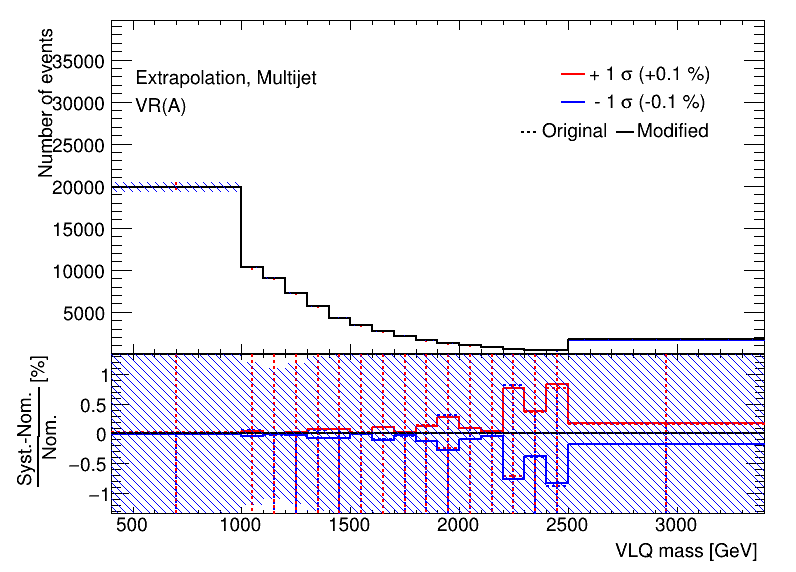
\includegraphics[width=\linewidth,height=\textheight,keepaspectratio]{VR_B_VLQM_Multijets.png}
			\caption{}
			\label{fig:uncertainties:systematics:btagging:extra:vlqm}
		\end{subfigure}
		\caption{Comparison between the Systematics-Nominal and Nominal, where Systematics-Nominal denotes the estimated multijet when both up (in red) and down (in blue) variations in \textit{extrapolation} are taken into account, and Nominal denotes the final estimated multijet (in black). The difference between the two is considered as the systematic uncertainty from the extrapolation of \pt. It is shown for (a) leading $b$-tagged jet \pt and (b) VLQ mass distribution.}
		\label{fig:uncertainties:systematics:btagging:extra}
	\end{figure}

	\item \textit{extrapolation\_c:} it describes the extrapolation uncertainty for $c$-jets mistagged as $b$-jets. Fig.\ \ref{fig:uncertainties:systematics:btagging:extra:c} shows the contribution of the extrapolation uncertainty from the mistagging of $c$-jets in \pt distribution of the leading $b$-jet and VLQ mass. These plots show that \textit{extrapolation\_c} uncertainty does not contribute to the difference in normalisation of the distributions.
	\begin{figure}[hbt!]
		\centering
		\graphicspath{{figs/chapter6/Systematics/Extrapolationfromcharm/}}
		\begin{subfigure}{.35\textwidth}
			\centering
			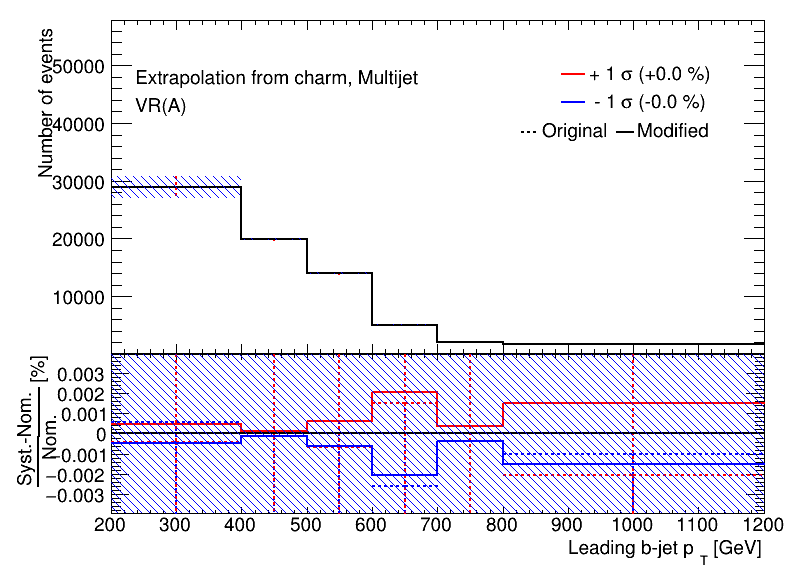
\includegraphics[width=\linewidth,height=\textheight,keepaspectratio]{VR_B_jet_pt_Multijets.png}
			\caption{}
			\label{fig:uncertainties:systematics:btagging:extra:c:jetpt}
		\end{subfigure}\hspace{0.6cm}
		\begin{subfigure}{.35\textwidth}
			\centering
			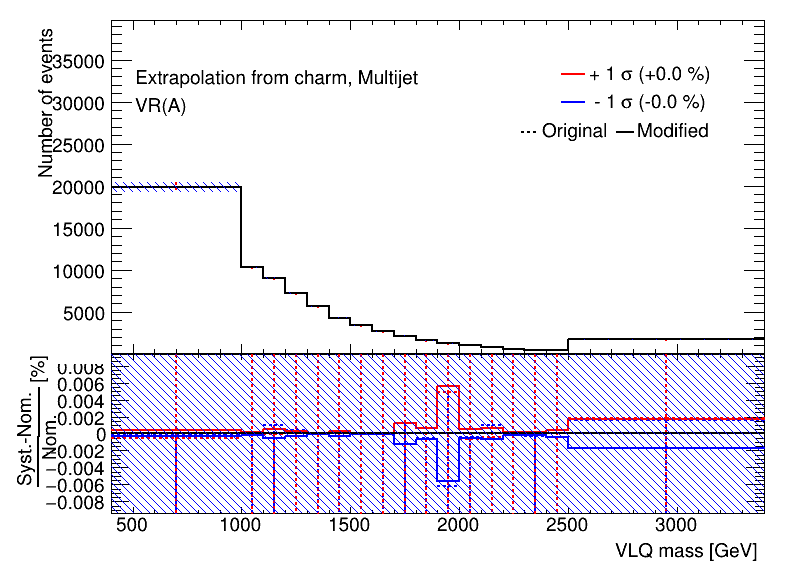
\includegraphics[width=\linewidth,height=\textheight,keepaspectratio]{VR_B_VLQM_Multijets.png}
			\caption{}
			\label{fig:uncertainties:systematics:btagging:extra:c:vlqm}
		\end{subfigure}
		\caption{Comparison between the Systematics-Nominal and Nominal, where Systematics-Nominal denotes the estimated multijet when both up (in red) and down (in blue) variations in \textit{extrapolation\_c} are taken into account, and Nominal denotes the final estimated multijet (in black). The difference between the two is considered as the systematic uncertainty from the extrapolation of \pt when $c$-jets are mistagged. It is shown for (a) leading $b$-tagged jet \pt and (b) VLQ mass distribution.}
		\label{fig:uncertainties:systematics:btagging:extra:c}
	\end{figure}
\end{itemize}

It was expected that the $b$-tagging uncertainties should be contributing the most because it is one of the uncorrelated variables which is used to define the ABCD regions. But however, the $b$-tagging uncertainties are only associated with the MC simulated backgrounds. The MC simulated backgrounds include multijet MC and the other MC backgrounds. The multijet MC is used for the calculation of \R, in which the likelihood fit is performed to fit the multijet MC to the data. The output of this fit, which is the scaled multijet MC, is used for the calculation of \R. In this, the likelihood fit constrains the $b$-tagging uncertainty in the scaled multijet MC. So, the contribution from the $b$-tagging uncertainty in the \R is suppressed, and the only contribution from the $b$-tagging uncertainty comes from the ABCD method, where the other MC backgrounds are used to subtract their contributions from the data according to Eqn.\ \ref{eqn:abcd:correctionfactor}. 

Also, $b$-tagging uncertainties contribute differently to all the six distributions because the likelihood fit and the calculation of the \R is performed separately for all the six distributions, but roughly it contributes to <1\% in the event yield of the multijet estimate in the validation region. Detailed values for all the distributions are given in Table \ref{table:uncertainties:systematics:detail}.


\begin{table}[hbt!]
	\centering
	\begin{tabular}{c|c|c|c|c|c|c} 
		\toprule
		Multijet & \multicolumn{3}{c}{$W$-tagged jet} \vline & \multicolumn{2}{c}{leading $b$-tagged jet} \vline & VLQ mass\\ \cline{2-6}
		Region A & \pt & mass & $\eta$ & \pt & mass & \\ 
		\midrule
		Est.\ Events & \num{72072} & \num{72752} & \num{72613} & \num{71670} & \num{73038} & \num{72573} \\
		Stat.\ uncertainty & $\pm$0.4\% & $\pm$0.5\% & $\pm$0.4\% & $\pm$2.6\% & $\pm$0.4\% & $\pm$0.8\% \\
		\midrule
		eigenvars\_b & $\pm$0.0\% & $\pm$0.0\% & $\pm$0.0\% & $\pm$0.0\% & $\pm$0.0\% & $\pm$0.0\% \\
		eigenvars\_c & $\pm$0.1\% & $\pm$0.0\% & $\pm$0.0\% & $\pm$0.1\% & $\pm$0.1\% & $\pm$0.0\% \\
		eigenvars\_light & $\pm$0.1\% & $\pm$0.1\% & $\pm$0.0\% & $\pm$0.2\% & $\pm$0.4\% & $\pm$0.1\% \\
		extrapolation & $\pm$0.1\% & $\pm$2.1\% & $\pm$0.1\% & $\pm$0.3\% & $\pm$1.2\% & $\pm$0.1\% \\
		extrapolation\_c & $\pm$0.0\% & $\pm$0.0\% & $\pm$0.0\% & $\pm$0.0\% & $\pm$0.0\% & $\pm$0.0\% \\
		\midrule
		Multijet MC & $\pm$3.8\% & $\pm$6.2\% & $\pm$4.4\% & $\pm$10.1\% & $\pm$4.6\% & $\pm$4.6\% \\
		Closure & $\pm$0.0\% & $\pm$0.0\% & $\pm$0.0\% & $\pm$0.0\% & $\pm$0.0\% & $\pm$0.0\% \\
		Cross-section & $\pm$0.2\% & $\pm$0.2\% & $\pm$0.2\% & $\pm$0.2\% & $\pm$0.2\% & $\pm$0.2\% \\
		\bottomrule
	\end{tabular}
	\caption{Overview of statistical and systematic uncertainties on the final estimated multijet when \R is calculated from the scaled multijet MC for all the six distributions.}
	\label{table:uncertainties:systematics:detail}
\end{table}


%==============================================================================
\subsection{Multijet MC uncertainty}
\label{sec:uncertainties:systematics:multijet}
%==============================================================================
As discussed before in section \ref{sec:abcd:correctionfactor}, the multijet estimate from the ABCD method where \R is calculated from the multijet MC samples (which are mismodelled) by using the bin-by-bin method can also be a result because it is also estimated from the same ABCD method. So, the difference between this estimate and the final estimate, which uses the scaled multijet MC for the calculation of \R is taken as multijet MC uncertainty. This uncertainty contributes a lot to the normalisation of the distribution. So, it is regarded as normalisation and shape uncertainty. The symmetry of multijet MC uncertainty is computed as one-sided since it only contributes towards the down variation and the up variation is added as the mirrored version of it. Fig.\ \ref{fig:uncertainties:systematics:multijet} shows the effect of this uncertainty in four different distributions. One can see that it adds differently to all the distributions in the validation region. Detailed values for all the distributions are given in Table \ref{table:uncertainties:systematics:detail}. The multijet MC uncertainty contributes most to the \pt distribution of the leading $b$-tagged jet where the first bin corresponds to almost 20\% uncertainty.

\begin{figure}[hbt!]
	\centering
	\graphicspath{{figs/chapter6/Systematics/PrefitBinbybin/}}
	\begin{subfigure}{.35\textwidth}
		\centering
		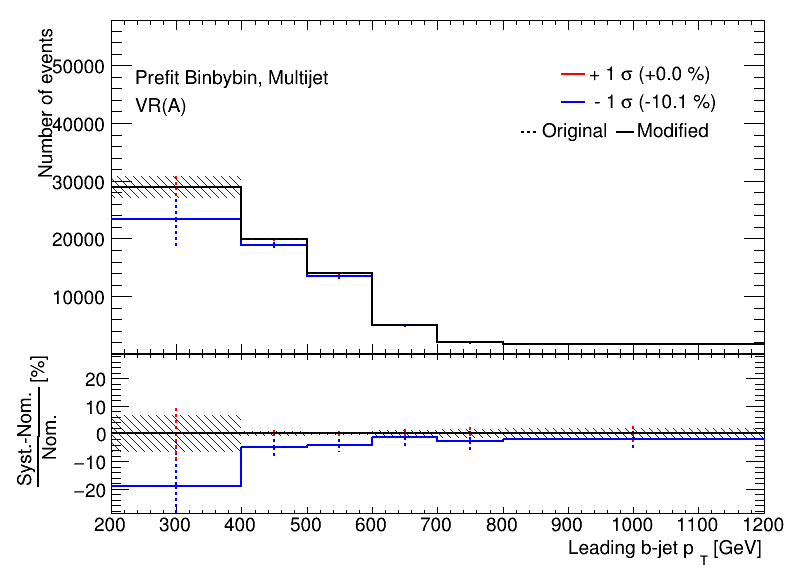
\includegraphics[width=\linewidth,height=\textheight,keepaspectratio]{VR_B_jet_pt_Multijets.png}
		\caption{}
		\label{fig:uncertainties:systematics:multijet:jetpt}
	\end{subfigure}\hspace{0.6cm}
	\begin{subfigure}{.35\textwidth}
		\centering
		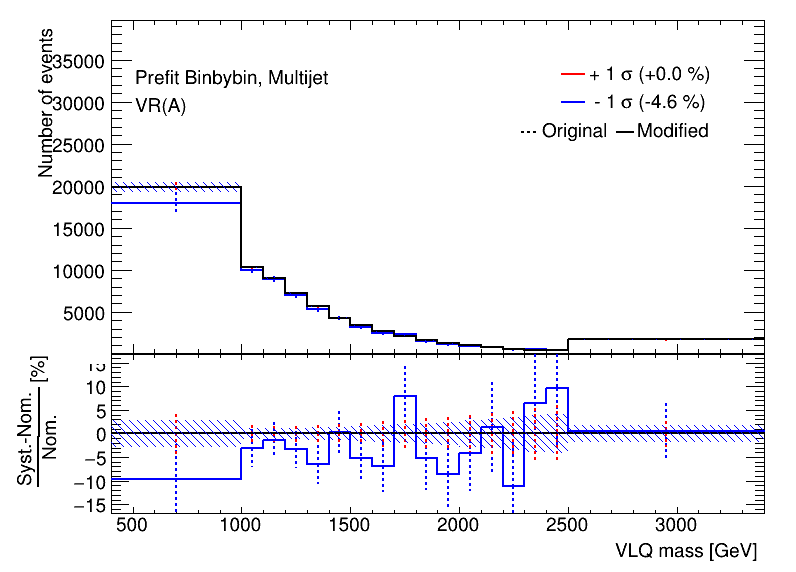
\includegraphics[width=\linewidth,height=\textheight,keepaspectratio]{VR_B_VLQM_Multijets.png}
		\caption{}
		\label{fig:uncertainties:systematics:multijet:vlqm}
	\end{subfigure}
	\begin{subfigure}{.35\textwidth}
		\centering
		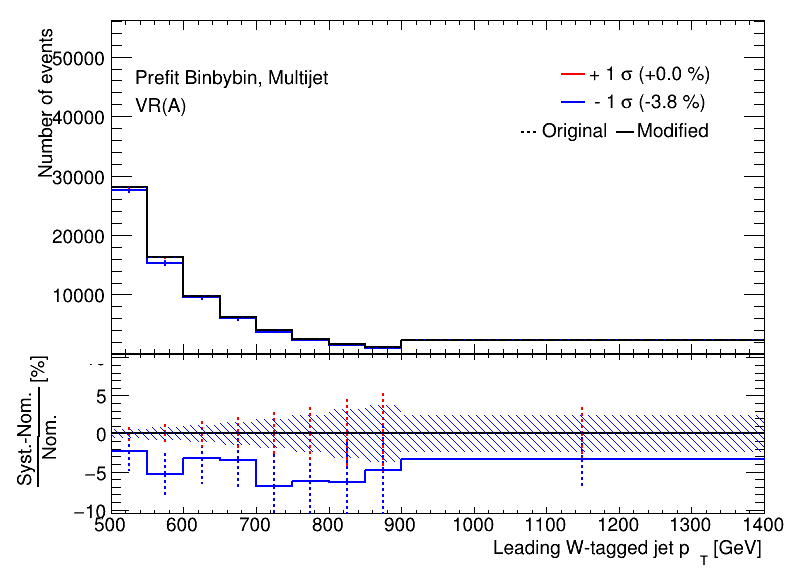
\includegraphics[width=\linewidth,height=\textheight,keepaspectratio]{VR_B_ljet_pt_Multijets.png}
		\caption{}
		\label{fig:uncertainties:systematics:multijet:ljetpt}
	\end{subfigure}\hspace{0.6cm}
	\begin{subfigure}{.35\textwidth}
		\centering
		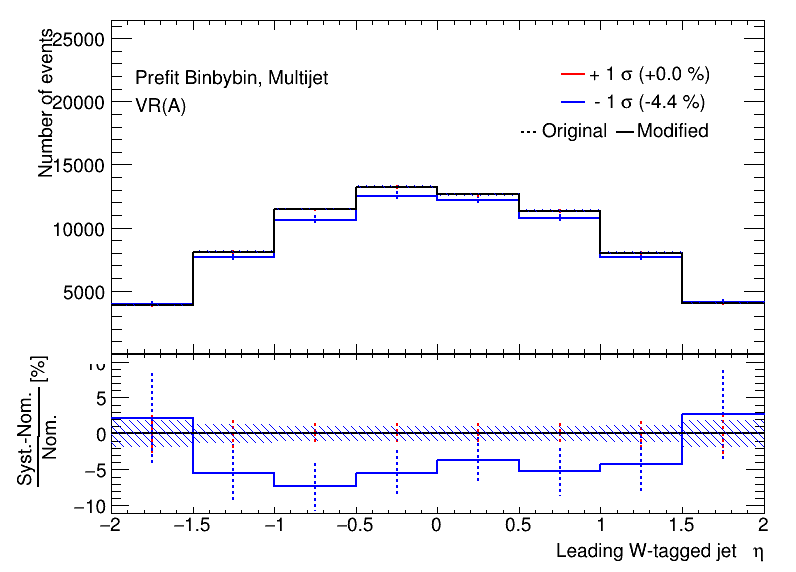
\includegraphics[width=\linewidth,height=\textheight,keepaspectratio]{VR_B_ljet_eta_Multijets.png}
		\caption{}
		\label{fig:uncertainties:systematics:multijet:ljeteta}
	\end{subfigure}
	\caption{Comparison between the Systematics-Nominal and Nominal, where Systematics-Nominal (in blue) denotes the estimated multijet when \R is calculated from the multijet MC (which are mismodelled), and Nominal denotes the final estimated multijet (in black) when \R is calculated from the scaled multijet MC. The difference between the two is considered as the multijet MC uncertainty. It is shown for (a) leading $b$-tagged jet \pt, (b) VLQ mass, (c) \pt and (d) $\eta$ distribution of leading $W$-tagged jet.}
	\label{fig:uncertainties:systematics:multijet}
\end{figure}


%==============================================================================
\subsection{Closure uncertainty}
\label{sec:uncertainties:systematics:closure}
%==============================================================================
In the closure uncertainty, the ABCD method is performed on the multijet MC instead of the data to estimate the multijet background in the validation region by using Eqn.\ \ref{eqn:uncertainties:systematics:closure}.
\begin{equation}
N_{\text{A}}^{\text{Est.\ multijet}}[i] = N_{\text{B}}^{\text{multijet MC}}[i] \times \frac{N_{\text{D}}^{\text{multijet MC}}[i]}{N_{\text{C}}^{\text{multijet MC}}[i]} \,,
\label{eqn:uncertainties:systematics:closure}
\end{equation}
where $N_{\text{j}}^{\text{Multijet MC}}[i]$ is event yield from the multijet MC in region j where j $\in$ \{B,C,D\}. Here [$i$] denotes that this calculation is performed bin-by-bin (where $i=$ bin).
 
Since multijet MC (which are mismodelled) are used for the multijet estimate, it is called MC-driven ABCD estimate instead of data-driven ABCD estimate. Here, data-driven ABCD estimate refers to the final multijet estimate when the \R is calculated from the scaled multijet MC by using the shape method. Note that there is no correction factor introduced in Eqn.\ \ref{eqn:uncertainties:systematics:closure} because previously in the data-driven ABCD estimate, the \R was calculated from the scaled multijet MC which was produced by performing a likelihood fit on the multijet MC. This cannot be performed in MC-driven ABCD estimate since the ABCD method itself is applied on the multijet MC. So, the normalisation of the MC-driven ABCD estimate would be less as compared to the normalisation of the data-driven ABCD estimate. Then, the normalisation of the MC-driven ABCD estimate is scaled to the normalisation of the data-driven ABCD estimate so that there would not be any difference in the normalisation of the two multijet estimates, but there would only be a shape variation. The difference in the shape of the distributions of the MC-driven ABCD estimate and the data-driven ABCD estimate is considered as the closure uncertainty. It is purely a shape uncertainty.

Fig.\ \ref{fig:uncertainties:systematics:closure} shows the effect of the closure uncertainty in four different distributions. The symmetry of the closure uncertainty is computed as one-sided since in some bins it contributes towards up variation, and in some bins, it contributes towards down variation as it can be noticed from the plots. One can observe a considerable shape variation in the \pt distribution of the leading $b$-jet, especially in the first bin where the difference is almost 100\%. This also shows how the \R corrects these bins where the difference is so significant.

\begin{figure}[hbt!]
	\centering
	\graphicspath{{figs/chapter6/Systematics/DijetsClosure/}}
	\begin{subfigure}{.35\textwidth}
		\centering
		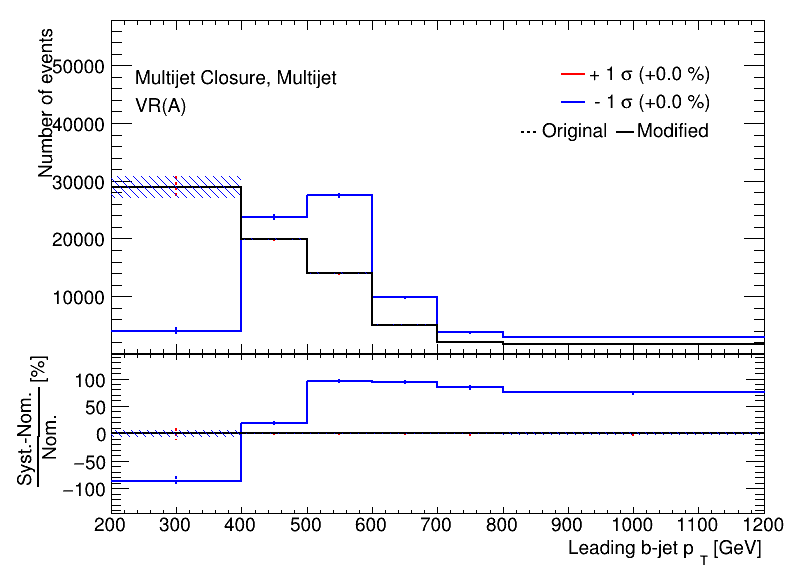
\includegraphics[width=\linewidth,height=\textheight,keepaspectratio]{VR_B_jet_pt_Multijets.png}
		\caption{}
		\label{fig:uncertainties:systematics:closure:jetpt}
	\end{subfigure}\hspace{0.6cm}
	\begin{subfigure}{.35\textwidth}
		\centering
		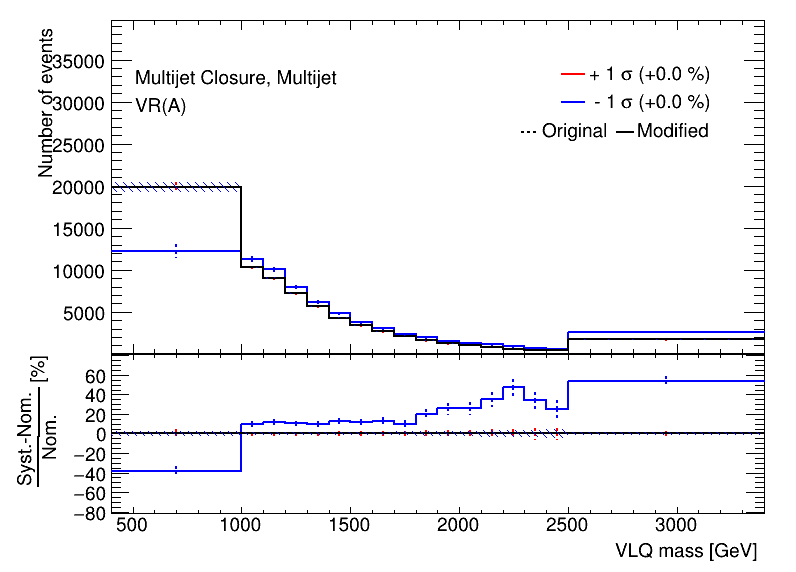
\includegraphics[width=\linewidth,height=\textheight,keepaspectratio]{VR_B_VLQM_Multijets.png}
		\caption{}
		\label{fig:uncertainties:systematics:closure:vlqm}
	\end{subfigure}
	\begin{subfigure}{.35\textwidth}
		\centering
		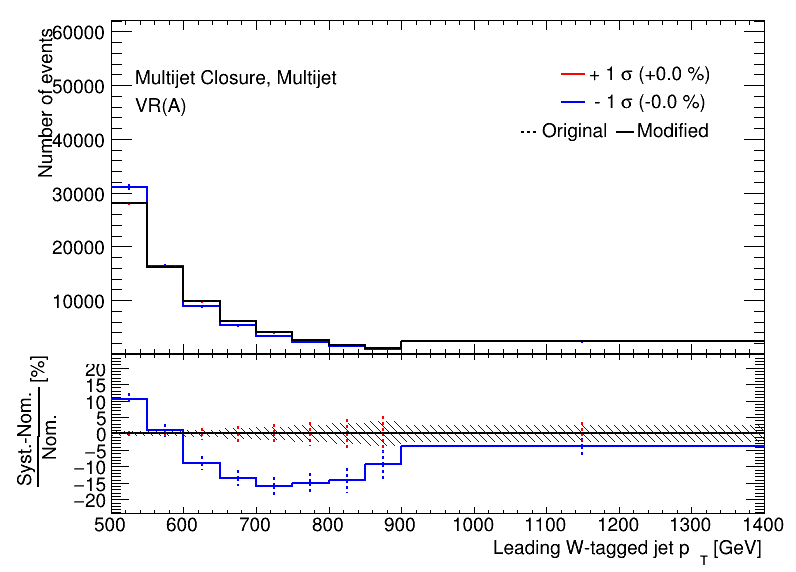
\includegraphics[width=\linewidth,height=\textheight,keepaspectratio]{VR_B_ljet_pt_Multijets.png}
		\caption{}
		\label{fig:uncertainties:systematics:closure:ljetpt}
	\end{subfigure}\hspace{0.6cm}
	\begin{subfigure}{.35\textwidth}
		\centering
		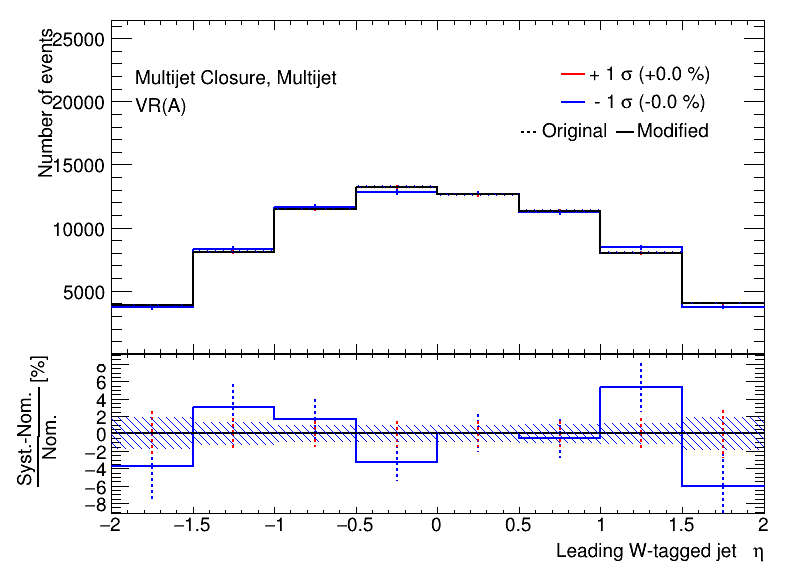
\includegraphics[width=\linewidth,height=\textheight,keepaspectratio]{VR_B_ljet_eta_Multijets.png}
		\caption{}
		\label{fig:uncertainties:systematics:closure:ljeteta}
	\end{subfigure}
	\caption{Comparison between the Systematics-Nominal and Nominal, where Systematics-Nominal (in blue) denotes the multijet from the MC-driven ABCD estimate, and Nominal denotes the final estimated multijet (in black) which is a data-driven ABCD estimate. The difference between the two is considered as the closure uncertainty. It is shown for (a) leading $b$-tagged jet \pt, (b) VLQ mass, (c) \pt and (d) $\eta$ distribution of leading $W$-tagged jet.}
	\label{fig:uncertainties:systematics:closure}
\end{figure}

%==============================================================================
\subsection{Cross-section uncertainty}
\label{sec:uncertainties:systematics:crossection}
%==============================================================================
The uncertainty in the values of a cross-section of different background processes is discussed in this section. The scale uncertainties on all background processes are given in Table \ref{table:uncertainties:systematics:crossection} by Physics Modelling Group (PMG)~\cite{crossection:top}~\cite{crossection:w}. 

\begin{table}[hbt!]
	\centering
	\begin{tabular}{c|c} 
		\toprule
		Background & Scale uncertainty \\ 
		\midrule
		Single top & $\pm$2.5\% \\
		$t\bar{t}$ & +2.4\% -3.5\% \\
		$W$+jets & $\pm$6\% \\
		$Z$+jets & $\pm$6\% \\
		\bottomrule
	\end{tabular}
	\caption{Scale uncertainty values for all the background processes.}
	\label{table:uncertainties:systematics:crossection}
\end{table}


Both up and down variations are taken into account by adding or subtracting the scale uncertainty on the cross-section of these backgrounds. Then, the ABCD method is performed in both the cases and the absolute mean of it is considered as the cross-section uncertainty. The scale uncertainty on the multijet MC is not taken into account since the ABCD estimate is only affected by the scale uncertainty on the cross-section of other backgrounds. Fig.\ \ref{fig:uncertainties:systematics:crossection} shows the impact of this uncertainty in four different distribution. It contributes to 0.2\% of an event yield of the multijet estimate in the validation region. Detailed values for all the distributions are given in Table \ref{table:uncertainties:systematics:detail}.

\begin{figure}[hbt!]
	\centering
	\graphicspath{{figs/chapter6/Systematics/Crossection/}}
	\begin{subfigure}{.35\textwidth}
		\centering
		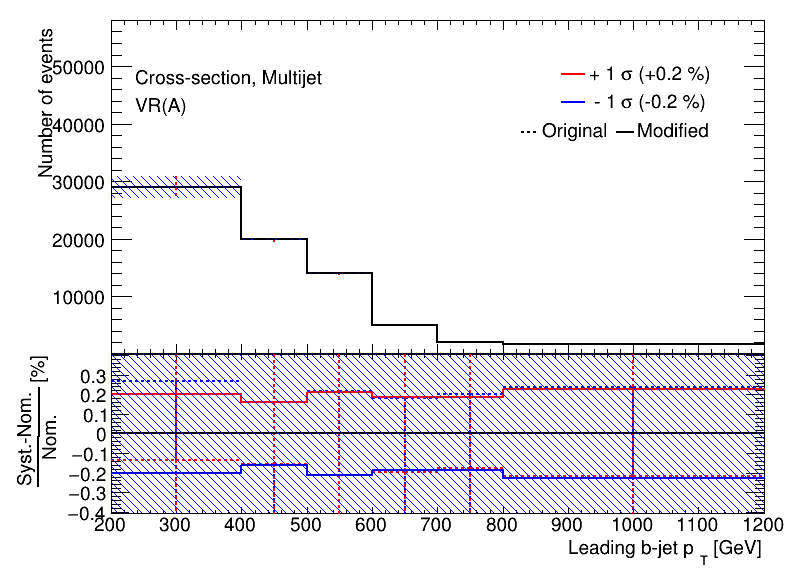
\includegraphics[width=\linewidth,height=\textheight,keepaspectratio]{VR_B_jet_pt_Multijets.png}
		\caption{}
		\label{fig:uncertainties:systematics:crossection:jetpt}
	\end{subfigure}\hspace{0.6cm}
	\begin{subfigure}{.35\textwidth}
		\centering
		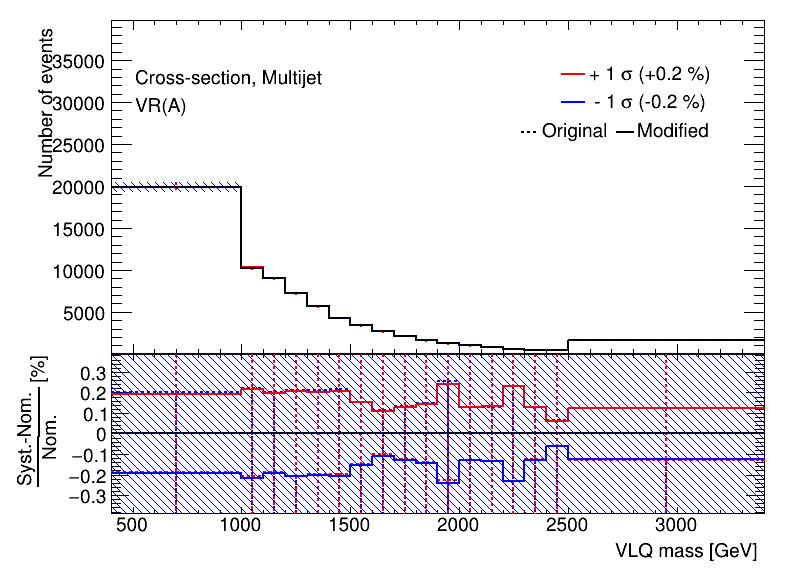
\includegraphics[width=\linewidth,height=\textheight,keepaspectratio]{VR_B_VLQM_Multijets.png}
		\caption{}
		\label{fig:uncertainties:systematics:crossection:vlqm}
	\end{subfigure}
	\begin{subfigure}{.35\textwidth}
		\centering
		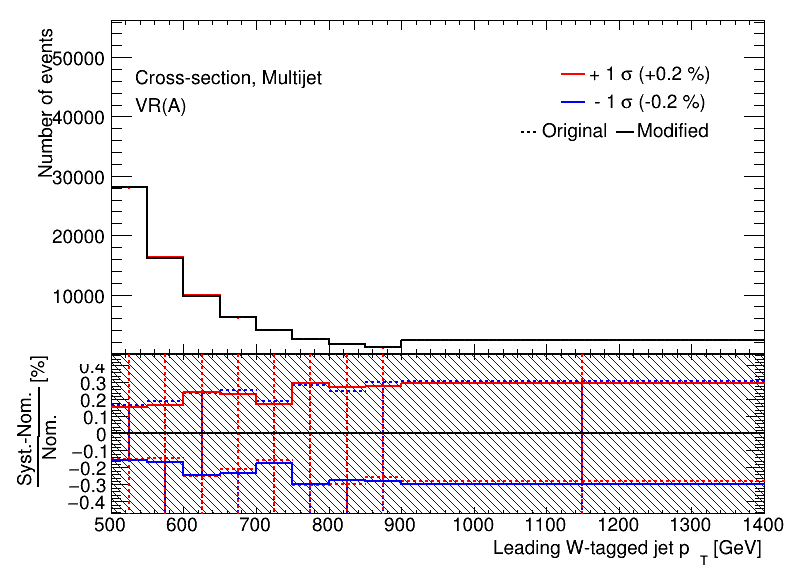
\includegraphics[width=\linewidth,height=\textheight,keepaspectratio]{VR_B_ljet_pt_Multijets.png}
		\caption{}
		\label{fig:uncertainties:systematics:crossection:ljetpt}
	\end{subfigure}\hspace{0.6cm}
	\begin{subfigure}{.35\textwidth}
		\centering
		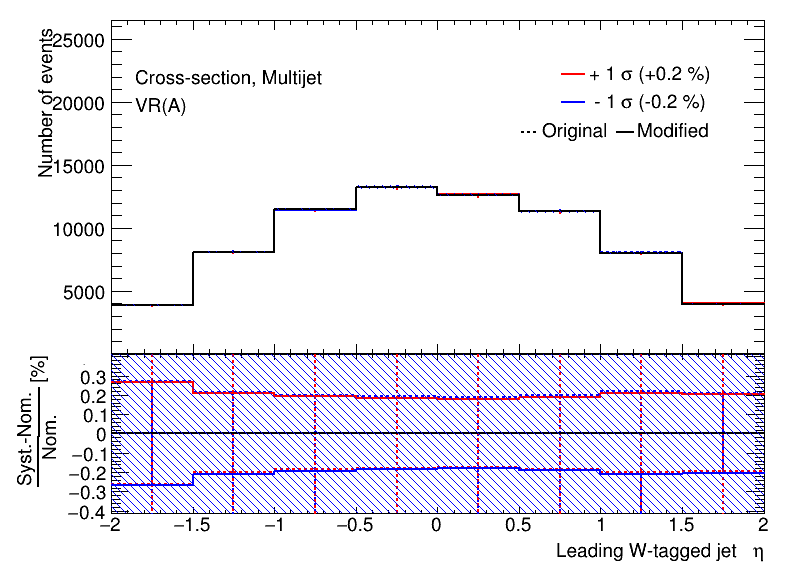
\includegraphics[width=\linewidth,height=\textheight,keepaspectratio]{VR_B_ljet_eta_Multijets.png}
		\caption{}
		\label{fig:uncertainties:systematics:crossection:ljeteta}
	\end{subfigure}
	\caption{Comparison between the Systematics-Nominal and Nominal, where Systematics-Nominal denotes the estimated multijet when both up (in red) and down (in blue) variations in cross-section uncertainties of all the other backgrounds are taken into account, and Nominal denotes the final estimated multijet (in black). The difference between the two is considered as the multijet MC  uncertainty. It is shown for (a) leading $b$-tagged jet \pt, (b) VLQ mass, (c) \pt and (d) $\eta$ distribution of leading $W$-tagged jet.}
	\label{fig:uncertainties:systematics:crossection}
\end{figure}


%%% Local Variables: 
%%% mode: latex
%%% TeX-master: "mythesis"
%%% End: 